% 2008 年新课标卷理科第 18 题：正方体 ABCD-A'B'C'D'，点 P 在对角线 BD' 上，∠PDA=60°。
% 来源 PDF：gaokaomath-src/普通高考/2008/2008新课标理(海南,宁夏).pdf
% SHA-256：e16be52b93c241bf45c4d6441855b577407007de032d2e902f11442c06ef66ec
% 原页：2008新课标理(海南,宁夏).pdf 第 1 页（A3 三栏）第 3 栏，书页码 467。
% 绘制依据：棱长取 1，斜投影 (x,y,z)->(x+0.5y, z+0.35y)；P 在 BD' 上（题面只给 ∠PDA=60°，
%   此处按解出的位置 t=2-√2 标在 BD' 上），BD' 与 DP 用虚线。被遮挡的 A—D、D—C、D—D' 亦为虚线。
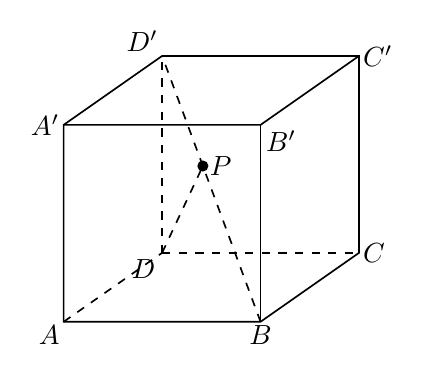
\begin{tikzpicture}[scale=2.5, semithick, every node/.style={inner sep=1.2pt}]
  \coordinate (A)  at (0.00,0.00);
  \coordinate (B)  at (1.00,0.00);
  \coordinate (C)  at (1.50,0.35);
  \coordinate (D)  at (0.50,0.35);
  \coordinate (Ap) at (0.00,1.00);
  \coordinate (Bp) at (1.00,1.00);
  \coordinate (Cp) at (1.50,1.35);
  \coordinate (Dp) at (0.50,1.35);
  \coordinate (P)  at (0.707,0.791);

  % 可见棱
  \draw (A) -- (B) -- (C) -- (Cp) -- (Dp) -- (Ap) -- cycle;
  \draw (B) -- (Bp);
  \draw (Ap) -- (Bp) -- (Cp);

  % 被遮挡的棱
  \draw[dashed] (A) -- (D);
  \draw[dashed] (D) -- (C);
  \draw[dashed] (D) -- (Dp);

  % 对角线 BD'、DP
  \draw[dashed] (B) -- (Dp);
  \draw[dashed] (D) -- (P);
  \fill (P) circle (0.8pt);

  \node[below left] at (A) {$A$};
  \node[below] at (B) {$B$};
  \node[right] at (C) {$C$};
  \node[below left=1pt] at (D) {$D$};
  \node[left] at (Ap) {$A'$};
  \node[below right=0.5pt] at (Bp) {$B'$};
  \node[right] at (Cp) {$C'$};
  \node[above left] at (Dp) {$D'$};
  \node[right=1pt] at (P) {$P$};
\end{tikzpicture}
